\section{HW3}
For each of the sentences below give an LF and derive the semantics of the sentence from this LF in the way we have been doing for the exercises on the 3d practice homework (that is, by assigning Lambda Calculus terms to the nodes of the LF tree).

In (2) and (5) only choose an LF for what you take to be the most plausible scope ordering.
\begin{QandA}
   \item Pedro owns a donkey. 
         \begin{answered}
			\begin{tikzpicture}[scale=1]
			\tikzset{level 1+/.style={level distance=30pt}}
			\tikzset{every tree node/.style={align=left,anchor=north}}
			\Tree [.S
			  [.DP Pedrow ]
			  [.VP
			    [.$V_{tr}$ owns ]
			    [.DP
			      [.Det a ]
			      [.NP donkey ] 
			    ]  
			  ] 
			]
         	\end{tikzpicture}
         	
			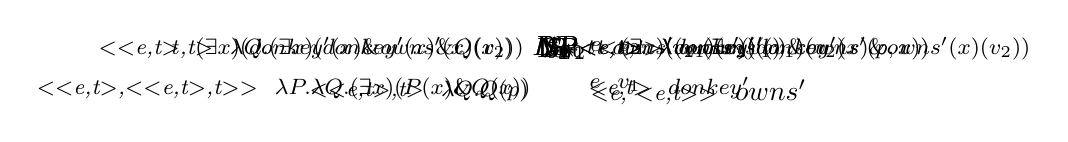
\begin{tikzpicture}[scale=0.7]
			\tikzset{level 1+/.style={level distance=30pt}}
			\tikzset{every tree node/.style={align=left,anchor=north}}
			\Tree [. \node[label={right:{\textit{\footnotesize t \space $(\exists x)(donkey'(x) \& owns'(p,x))$}}}]{$S \star$};
			  [. \node[label={below left:\textit{ \footnotesize $<<$e,t$>$,t$>$ \space $\lambda Q. Q(p)$}}]{$DP_2$}; Pedro ]
			     [.\node[label={right:\textit{\footnotesize $<$e,t$>$ \space $\lambda v_2. (\exists x)(donkey'(x) \& owns'(x)(v_2))$}}]{}; 
			       [.2 ] 
			       [.\node[label={left:\textit{\footnotesize t \space $(\exists x)(donkey'(x) \& owns'(x)(v_2))$}}]{$S \ast$};
			         [.\node[label={left:\textit{\footnotesize $<<$e,t$>$,t$>$ \space $\lambda Q. (\exists x)(donkey'(x) \& Q(x))$}}]{$DP_1$}; 
			           [.\node[label={below left:\textit{\footnotesize $<<$e,t$>$,$<<$e,t$>$,t$>>$ \space $\lambda P. \lambda Q. (\exists x)(P(x) \& Q(x))$ }}]{Det}; a ]
			           [.\node[label={below right:\textit{\footnotesize $<$e,t$>$ \space $donkey'$}}]{NP}; donkey ]
			         ]
			         [.\node[label={right:\textit{\footnotesize $<$e,t$>$ \space $\lambda v_1 . owns'(v_1)(v_2)$}}]{};
			           [.1 ]
			           [.\node[label={right:\textit{\footnotesize $t$ \space $owns'(v_1)(v_2)$}}]{S};
			             [.\node[label={right:\textit{\footnotesize $e$ \space $v_2$ }}]{$t_2$};]
			             [.\node[label={right:\textit{\footnotesize $<$e,t$>$ \space $owns'(v_1)$ }}]{VP};
			               [.\node[label={below right:\textit{\footnotesize $<$e, $<$e,t$>$$>$} \space $owns'$}]{$V_{tr}$}; owns ]
			               [.\node[label={below right:\textit{\footnotesize $e$ \space $v_1$ }}]{$t_1$};]
			             ]
			           ]
			         ]
			       ]
			     ]
			  ]
			\end{tikzpicture}
 		 \begin{align*}
 		 \ast & =\lambda Q. (\exists x)(donkey'(x) \& Q(x))(\lambda v_1 owns'(v_1)(v_2)) \\
 		 & = (\exists x)(donkey'(x) \& (\lambda v_1 owns'(v_1)(v_2))(x)) \\
 		 & = (\exists x)(donkey'(x) \& owns'(x)(v_2)) \\ \\
 		 \star & =(\lambda Q. Q(j))(\lambda v_2. (\exists x)(donkey'(x) \& owns'(x)(v_2))) \\
 		 & = (\lambda v_2.(\exists x)(donkey'(x) \& owns'(x)(v_2)))(p) \\
 		 & = (\exists x)(donkey'(x) \& owns'(x)(p)) \\
 		 & = (\exists x)(donkey'(x) \& owns'(p,x))
 		 \end{align*}

         \end{answered}

   \item Somebody likes nobody.
         \begin{tikzpicture}[scale=1]
   			\tikzset{level 1+/.style={level distance=30pt}}
   			\tikzset{every tree node/.style={align=left,anchor=north}}
   			\Tree [.S
   			  [.DP Somebody ]
   			  [.VP
   			    [.$V_{tr}$ likes ]
   			    [.DP nobody ]  
   			  ] 
   			]
         \end{tikzpicture}
   
         \begin{answered}
			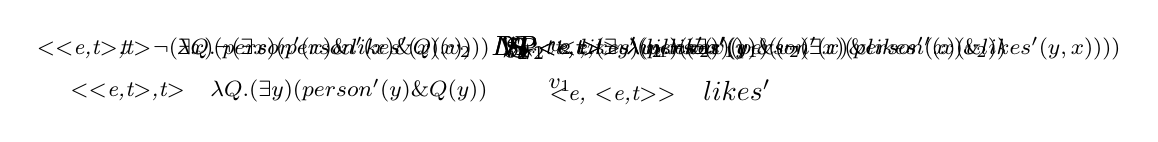
\begin{tikzpicture}[scale=0.75]
			\tikzset{level 1+/.style={level distance=30pt}}
			\tikzset{every tree node/.style={align=left,anchor=north}}
			\Tree [. \node[label={right:{\textit{\footnotesize t \space;\space $(\exists y)(person'(y) \& (\neg (\exists x)(person'(x) \& likes'(y,x))))$}}}]{$S \star$};
			  [. \node[label={below left:\textit{ \footnotesize $<<$e,t$>$,t$>$ \space\space $\lambda Q. (\exists y)(person'(y) \& Q(y))$}}]{$DP_2$}; Somebody ]
			     [.\node[label={right:\textit{\footnotesize $<$e,t$>$ \space\space $\lambda v_2. \neg (\exists x)(person'(x) \& likes'(x)(v_2))$}}]{}; 
			       [.2 ] 
			       [.\node[label={left:\textit{\footnotesize t \space\space $\neg (\exists x)(person'(x) \& likes'(x)(v_2))$}}]{$S$};
			         [.\node[label={left:\textit{\footnotesize $<<$e,t$>$,t$>$ \space\space $\lambda Q. \neg (\exists x)(person'(x) \& Q(x))$}}]{$DP_1$}; nobody ]
			         [.\node[label={right:\textit{\footnotesize $<$e,t$>$ \space\space $\lambda v_1 . likes'(v_1)(v_2)$}}]{};
			           [.1 ]
			           [.\node[label={right:\textit{\footnotesize $t$ \space\space $likes'(v_1)(v_2)$}}]{S};
			             [.\node[label={right:\textit{\footnotesize $v_2$ }}]{$t_2$};]
			             [.\node[label={right:\textit{\footnotesize $<$e,t$>$ \space\space $likes'(v_1)$ }}]{VP};
			               [.\node[label={below right:\textit{\footnotesize $<$e, $<$e,t$>$$>$} \space\space $likes'$}]{$V_{tr}$}; likes ]
			               [.\node[label={below right:\textit{\footnotesize $v_1$ }}]{$t_1$};]
			             ]
			           ]
			         ]
			       ]
			     ]
			  ]
			\end{tikzpicture}
			\begin{align*}
	 		 \star & =(\lambda Q. (\exists y)(person'(y) \& Q(y)))(\lambda v_2. \neg (\exists x)(person'(x) \& likes'(x)(v_2))) \\
	 		 & = (\exists y)(person'(y) \& (\lambda v_2. \neg (\exists x)(person'(x) \& likes'(x)(v_2))(y))) \\
	 		 & = (\exists y)(person'(y) \& (\neg (\exists x)(person'(x) \& likes'(x)(y)))) \\
	 		 & = (\exists y)(person'(y) \& (\neg (\exists x)(person'(x) \& likes'(y,x))))
			\end{align*}
         \end{answered}
         
   \item Every sensible person who likes Mozart likes Haydn.
         \begin{answered}
         \begin{tikzpicture}[scale=1]
   			\tikzset{level 1+/.style={level distance=30pt}}
   			\tikzset{every tree node/.style={align=left,anchor=north}}
   			\Tree [.S
   			  [.DP 
   			    [.Det every ]
   			    [.NP
   			      [.AP sensible ]
   			      [.NP
   			        [.NP person ]
   			        [.RC
   			          [.Comp who ]
   			          [.VP
   			            [.$V_{tr}$ likes ]
   			            [.DP Mozart ] 
   			          ]
   			        ] 
   			      ] 
   			    ]
   			  ]
   			  [.VP
   			    [.$V_{tr}$ likes ]
   			    [.DP Haydn ]  
   			  ] 
   			]
         \end{tikzpicture}
         
		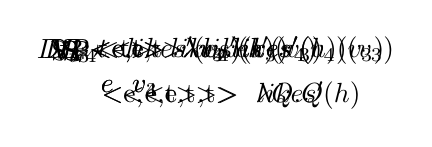
\begin{tikzpicture}[scale=0.8]
		\Tree [.\node {S $\ast$};
		        [.\node(site){$DP_3 \star$}; ]
		        [.\node [label={right: $<$e,t$>$ \space $\lambda v_3. likes'(h)(v_3)$}]{}; 
		          [.3 ]
		          [.\node [label={right: $<$t$>$ \space $likes'(h)(v_3)$}] {S};
		            [.\node [label={below right: $<<$e,t$>$,t$>$ \space $\lambda Q. Q(h)$}] {$DP_4$}; Hayden ]
		            [.\node [label={right: $<$e,t$>$ \space $\lambda v_4. likes'(v_4)(v_3)$}] {};
		              [.4 ]
		              [.\node [label={right: $t$ \space $likes'(v_4)(v_3)$}] {S}; 
		                [.\node [label={below right: $e$ \space $v_3$}] {$t_3$}; ]
		                [.\node [label={right: $<$e,t$>$ \space $likes'(v_4)$}] {VP};
		                  [.\node [label={below right: $<$e,$<$e,t$>>$ \space $likes'$}] {$V_{tr}$}; likes ]
		                  [.\node [label={below right: $e$ \space $v_4$}] {$t_4$}; ]
		                ]
		              ]
		            ]
		          ]
		        ]
		      ]
		\end{tikzpicture}
		
		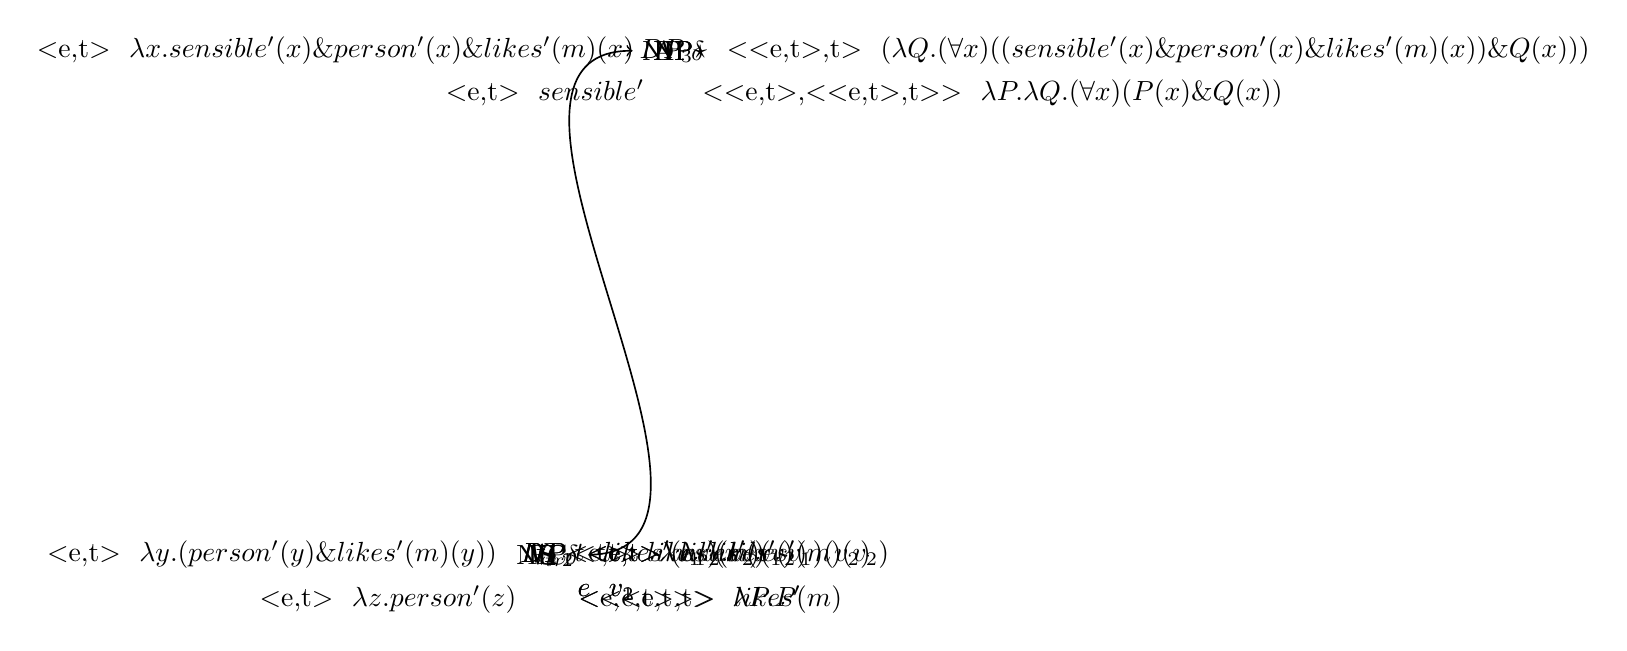
\begin{tikzpicture}[scale=0.8]
		\tikzset{level 1+/.style={level distance=30pt}}
		\tikzset{every tree node/.style={align=left,anchor=north}}
		\begin{scope}
		\Tree [.\node [label={right: $<<$e,t$>$,t$>$ \space $(\lambda Q. (\forall x)((sensible'(x) \& person'(x) \& likes'(m)(x)) \& Q(x)))$ }] {$DP_3 \star$}; 
		        [.\node [label={below right: $<<$e,t$>$,$<<$e,t$>$,t$>>$ \space $\lambda P. \lambda Q. (\forall x)(P(x) \& Q(x))$ }] {DP}; every ]
		        [.\node [label={left: $<$e,t$>$ \space $\lambda x. sensible'(x) \& person'(x) \& likes'(m)(x)$}] {NP};
		          [.\node(empty){NP $\delta$}; ]
		          [.\node [label={below left: $<$e,t$>$ \space $sensible'$}] {AP}; sensible ]
%		          [.\node [label={right: $<$e,t$>$ \space $\lambda y. (person'(y) \& likes'(m)(y))$}] {NP};
%		            [.\node [label={below right: $<$e,t$>$ \space $person'$}] {$NP_2$}; person ]
%		            [.\node [label={right: $<$e,t$>$ \space $\lambda v_2. likes'(m)(v_2)$}] {RC}; 
%		              [.COMP who ]
%		              [.\node [label={right: $<$t$>$ \space $likes'(m)(v_2)$}] {S};
%		                [.\node [label={below right: $<<$e,t$>$,t$>$ \space $\lambda P. P(m)$}] {$DP_1$}; Mozart ]
%		                [.\node(empty) [label={right: $<$e,t$>$ \space $\lambda v_1. likes'(v_1)(v_2)$}] {};
%		                  [.1 ]
%		                  [.\node [label={right: $t$ \space $likes'(v_1)(v_2)$}] {S};
%		                    [.\node [label={below right: $e$ \space $v_2$}] {$t_2$}; ]
%		                    [.\node [label={right: $<$e,t$>$ \space $likes'(v_1)$}] {VP};
%		                      [.\node [label={below right: $<$e,$<$e,t$>>$ \space $likes'$}] {$V_{tr}$}; likes ]
%		                      [.\node [label={below right: $e$ \space $v_1$}] {$t_1$}; ]
%		                    ]
%		                  ]
%		                ]
%		              ]
%		            ]
%		          ]
		        ]
		      ]
		\end{scope}
		\begin{scope}[shift=({-2cm, -8cm})]
        \Tree [.\node (root) [label={left: $<$e,t$>$ \space $\lambda y. (person'(y) \& likes'(m)(y))$}] {NP $\delta$};
        		            [.\node [label={below left: $<$e,t$>$ \space $\lambda z. person'(z)$}] {$DP_2$}; person ]
        		            [.\node [label={right: $<$e,t$>$ \space $\lambda v_2. likes'(m)(v_2)$}] {RC}; 
        		              [.COMP who ]
        		              [.\node [label={right: $<$t$>$ \space $likes'(m)(v_2)$}] {S};
        		                [.\node [label={below right: $<<$e,t$>$,t$>$ \space $\lambda P. P(m)$}] {$DP_1$}; Mozart ]
        		                [.\node [label={right: $<$e,t$>$ \space $\lambda v_1. likes'(v_1)(v_2)$}] {};
        		                  [.1 ]
        		                  [.\node [label={right: $t$ \space $likes'(v_1)(v_2)$}] {S};
        		                    [.\node [label={below right: $e$ \space $v_2$}] {$t_2$}; ]
        		                    [.\node [label={right: $<$e,t$>$ \space $likes'(v_1)$}] {VP};
        		                      [.\node [label={below right: $<$e,$<$e,t$>>$ \space $likes'$}] {$V_{tr}$}; likes ]
        		                      [.\node [label={below right: $e$ \space $v_1$}] {$t_1$}; ]
        		                    ]
        		                  ]
        		                ]
        		              ]
        		            ]
        		          ]
		\end{scope}
		\draw[semithick,->] (root) to [out=0, in=180] (empty);
		\end{tikzpicture}
		
		\begin{align*}
		\delta & = (\lambda P. \lambda Q. \lambda y. (P(y) \& Q(y)))(\lambda v_2. likes'(m)(v_2))(\lambda z. person'(z)) \\
		& = (\lambda Q. \lambda y. ((\lambda z. person'(z))(y) \& Q(y)))(\lambda v_2. likes'(m)(v_2)) \\
		& = (\lambda Q. \lambda y. (person'(y) \& Q(y)))(\lambda v_2. likes'(m)(v_2)) \\
		& = \lambda y. (person'(y) \& (\lambda v_2. likes'(m)(v_2))(y)) \\
		& = \lambda y. (person'(y) \& likes'(m)(y))
		\end{align*}
		\begin{align*}
 		\star & =\lambda P. \lambda Q. (\forall x)(P(x) \& Q(x)))(\lambda x. sensible'(x) \& person'(x) \& likes'(m)(x) \\
 		& =  \lambda Q. (\forall x)((\lambda x. sensible'(x) \& person'(x) \& likes'(m)(x))(x) \& Q(x))\\
 		& = \lambda Q. (\forall x)((sensible'(x) \& person'(x) \& likes'(m)(x)) \& Q(x)) \\
 		\end{align*}
 		\begin{align*}
 		\ast & =\lambda Q. (\forall x)((sensible'(x) \& person'(x) \& likes'(m)(x)) \& Q(x)))(\lambda v_3. likes'(h)(v_3)) \\
 		& =  (\forall x)(sensible'(x) \& person'(x) \& likes'(m)(x) \& likes'(h)(x))\\
		\end{align*}
         
         \end{answered}
   \item An American farmer talked to a Canadian farmer. (Treat ‘talk to’ as a transitive verb.)
         \begin{answered}
         \begin{tikzpicture}[scale=1]
 			\tikzset{level 1+/.style={level distance=30pt}}
 			\tikzset{every tree node/.style={align=left,anchor=north}}
 			\Tree [.S
   			        [.DP 
   			          [.Det An ]
   			          [.NP
   			            [.AP American ]
   			            [.NP farmer ] 
   			          ]
   			        ]
   			        [.VP
   			          [.$V_{tr}$ {talked to} ]
   			          [.DP
   			            [.Det a ]
   			            [.NP
   			              [.AP Canadian ]
   			              [.NP farmer ]
   			            ]
   			          ]
   			        ]
   			]
        \end{tikzpicture}
        
      	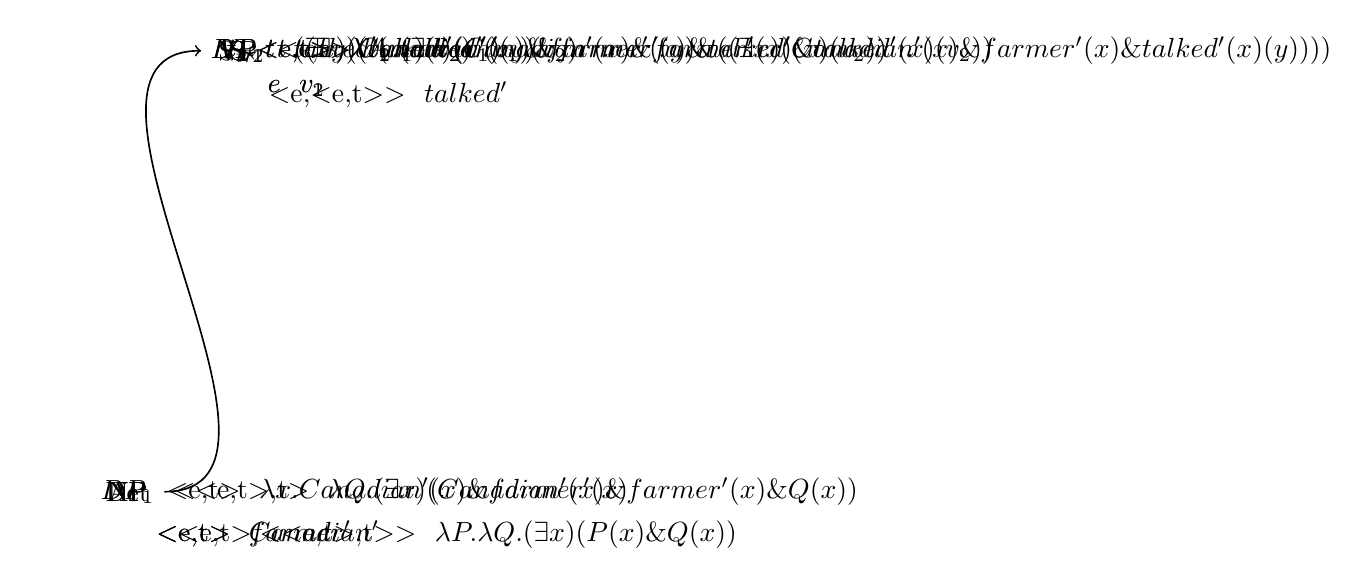
\begin{tikzpicture}[scale=0.7]
        \Tree [.\node [label={right: $t$ \space $(\exists y)(American'(y) \& farmer'(y) \& ((\exists x)(Canadian'(x) \& farmer'(x) \& talked'(x)(y))))$}] {S $\star$}; 
                [.\node {$DP_2$}; ]
                [.\node [label={right: $<$e,t$>$ \space $\lambda v_2. (\exists x)(Canadian'(x) \& farmer'(x) \& talked'(x)(v_2))$}] {}; 
                  [.2 ]
                  [.\node [label={right: $t$ \space $(\exists x)(Canadian'(x) \& farmer'(x) \& talked'(x)(v_2))$}] {S}; 
                    [.\node(dp1-o) {$DP_1$}; ]
                    [.\node [label={right: $<$e,t$>$ \space $\lambda v_1. talked'(v_1)(v_2)$}] {};
                      [.1 ]
                      [.\node [label={right: $t$ \space $talked'(v_1)(v_2)$}] {S}; 
                        [.\node [label={below right: $e$ \space $v_2$}] {$t_2$}; ]
                        [.\node [label={right: $<$e,t$>$ \space $talked'(v_1)$}] {VP}; 
                          [.\node [label={below right: $<$e,$<$e,t$>>$ \space $talked'$}]{$V_{tr}$}; ]
                          [.\node [label={below right: $e$ \space $v_1$}] {$t_1$}; ]
                        ]
                      ] 
                    ]
                  ]
                ]
              ]
        \begin{scope}[shift=({-2cm, -8cm})]
        \Tree [.\node (dp1) [label={right: $<<$e,t$>$,t$>$ \space $\lambda Q. (\exists x)(Canadian'(x) \& farmer'(x) \& Q(x))$}] {$DP_1$}; 
                [.\node [label={below right: $<<$e,t$>$,$<<$e,t$>$,t$>>$ \space $\lambda P. \lambda Q. (\exists x)(P(x) \& Q(x))$}] {Det}; a ]
                [.\node [label={right: $<$e,t$>$ \space $\lambda x. Canadian'(x) \& farmer'(x)$}] {NP}; 
                  [.\node [label={below right: $<$e,t$>$ \space $Canadian'$}] {AP}; Canadian ]
                  [.\node [label={below right: $<$e,t$>$ \space $farmer'$}] {NP}; farmer ]
                ]
              ]
        \end{scope}
        \draw[semithick,->] (dp1) to [out=0, in=180] (dp1-o);
      	\end{tikzpicture}
      	
      	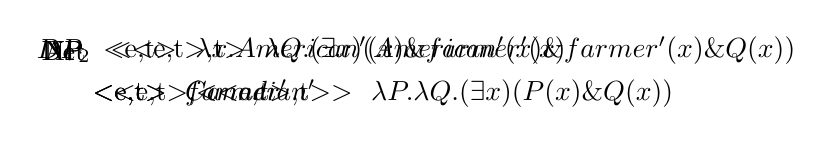
\begin{tikzpicture}[scale=0.7]
       \Tree [.\node (dp2) [label={right: $<<$e,t$>$,t$>$ \space $\lambda Q. (\exists x)(American'(x) \& farmer'(x) \& Q(x))$}] {$DP_2$}; 
               [.\node [label={below right: $<<$e,t$>$,$<<$e,t$>$,t$>>$ \space $\lambda P. \lambda Q. (\exists x)(P(x) \& Q(x))$}] {Det}; an ]
               [.\node [label={right: $<$e,t$>$ \space $\lambda x. American'(x) \& farmer'(x)$}] {NP}; 
                 [.\node [label={below right: $<$e,t$>$ \space $Canadian'$}] {AP}; American ]
                 [.\node [label={below right: $<$e,t$>$ \space $farmer'$}] {NP}; farmer ]
               ]
             ]      	
      	\end{tikzpicture}
      	
    	\begin{align*}
    	 \star & =\lambda Q. (\exists y)(American'(y) \& farmer'(y) \& Q(y))(\lambda v_2 (\exists x)(Canadian'(x) \& farmer'(x) \& talked'(x)(v_2))) \\
    	 & =  (\exists y)(American'(y) \& farmer'(y) \& (\lambda v_2 (\exists x)(Canadian'(x) \& farmer'(x) \& talked'(x)(v_2)))(y))\\
    	 & =  (\exists y)(American'(y) \& farmer'(y) \& ((\exists x)(Canadian'(x) \& farmer'(x) \& talked'(x)(y))))\\
    	 \end{align*}

        \end{answered}
   \item Not everybody who likes somebody likes everybody. (N.B. In (5) treat ‘not everybody’ as an unanalyzed determiner with the semantics:
   $\lambda P. \lambda Q. \neg (\forall x)(P(x)\rightarrow Q(x))$)
         \begin{answered}
         \begin{tikzpicture}[scale=1]
   			\tikzset{level 1+/.style={level distance=30pt}}
   			\tikzset{every tree node/.style={align=left,anchor=north}}
   			\Tree [.S
   			  [.DP 
   			    [.Det {not everybody} ]
   			    [.RC
   			      [.Comp who ]
   			      [.VP
   			        [.{$V_{tr}$} likes ]
   			        [.DP Somebody ]
   			      ] 
   			    ] 
   			  ]
   			  [.VP
   			    [.$V_{tr}$ likes ]
   			    [.DP everybody ]  
   			  ] 
   			]
         \end{tikzpicture}
         
         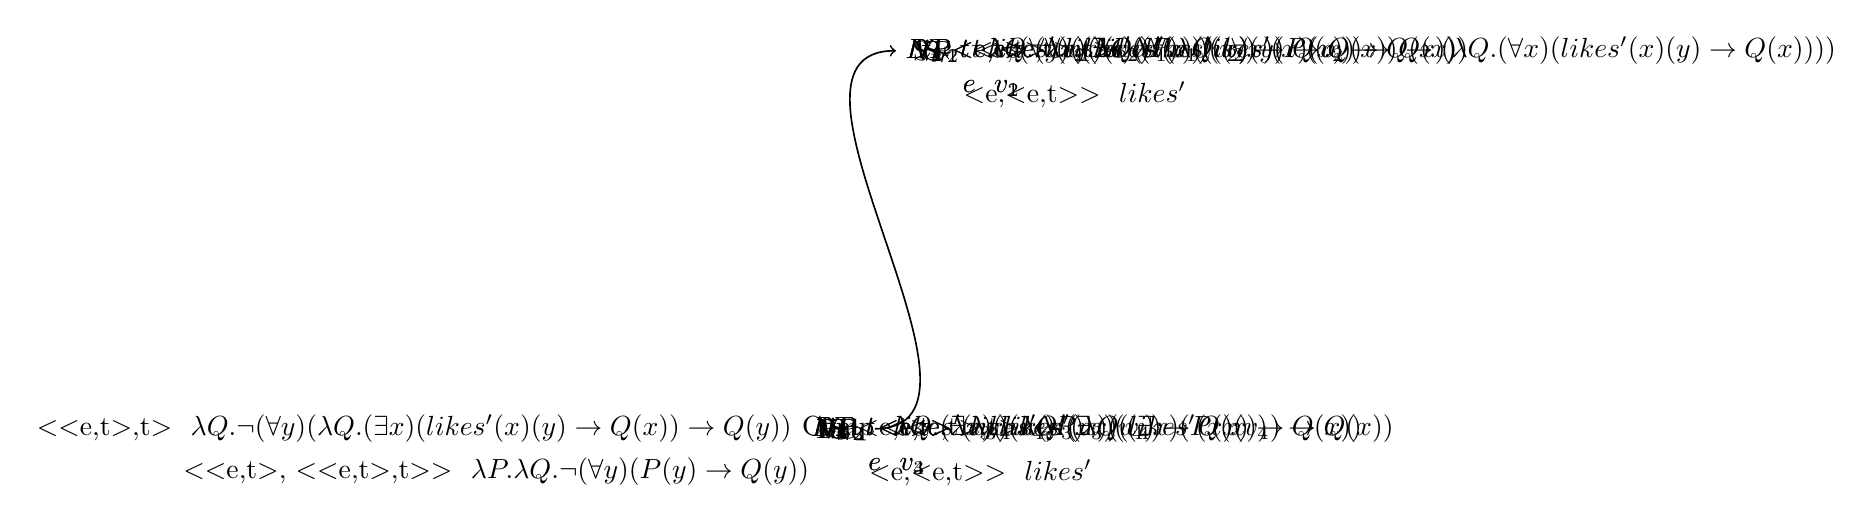
\begin{tikzpicture}[scale=0.6]
         \Tree [.\node [label={right: $t$ \space $\neg (\forall y)((\exists x) (likes'(x)(y) \rightarrow Q(x))\rightarrow (\lambda Q. (\forall x)(likes'(x)(y)\rightarrow Q(x))))$}] {S $\star$}; 
                 [.\node(dp2-o) {$DP_2$}; ]
                 [.\node [label={right: $<$e,t$>$ \space $\lambda v_2. \lambda Q. (\forall x)(likes'(x)(v_2)\rightarrow Q(x))$}] {};
                   [.2 ]
                   [.\node [label={right: $t$ \space $\lambda Q. (\forall x)(likes'(x)(v_2)\rightarrow Q(x))$}] {S};
                     [.\node [label={right: $<<$e,t$>$,t$>$ \space $\lambda P. \lambda Q. (\forall x)(P(x)\rightarrow Q(x))$}] {$DP_1$}; everybody ]
                     [.\node [label={right: $<$e,t$>$ \space $\lambda v_1. likes'(v_1)(v_2)$}] {};
                       [.1 ]
                       [.\node [label={right: $t$ \space $likes'(v_1)(v_2)$}] {S}; 
                         [.\node [label={below right: $e$ \space $v_2$}] {$t_2$}; ]
                         [.\node [label={right: $<$e,t$>$ \space $likes'(v_1)$}] {VP}; 
                           [.\node [label={below right: $<$e,$<$e,t$>>$ \space $likes'$}] {$V_{tr}$}; ]
                           [.\node [label={below right: $e$ \space $v_1$}] {$t_1$}; ]
                         ]
                       ]
                     ]
                   ]
                 ]
               ]
         \begin{scope}[shift=({-2cm, -8cm})]
         \Tree [.\node (dp2) [label={left: $<<$e,t$>$,t$>$ \space $\lambda Q. \neg (\forall y)(\lambda Q. (\exists x) (likes'(x)(y) \rightarrow Q(x))\rightarrow Q(y))$}] {$DP_2$}; 
                 [.\node [label={below left: $<<$e,t$>$, $<<$e,t$>$,t$>>$ \space $\lambda P. \lambda Q. \neg (\forall y)(P(y)\rightarrow Q(y))$}] {Det}; {not everybody} ]
                 [.\node [label={right: $<$e,t$>$ \space $\lambda v_4. \lambda Q. (\exists x) (likes'(x)(v_4) \rightarrow Q(x))$}] {RC}; 
                   [.\node {Comp}; who ] 
                   [.\node [label={right: $t$ \space $\lambda Q. (\exists x) (likes'(x)(v_4) \rightarrow Q(x))$}] {S}; 
                       [.\node [label={right: $<<$e,t$>$,t$>$ \space $\lambda P. \lambda Q. (\exists x) (P(x) \rightarrow Q(x))$}] {$DP_3$}; somebody ]
                       [.\node [label={right: $<$e,t$>$ \space $\lambda v_3. likes'(v_3)(v_4)$}] {}; 
                         [.3 ]
                         [.\node [label={right: $t$ \space $likes'(v_3)(v_4)$}]{S};
                           [.\node [label={below right: $e$ \space $v_4$}] {$t_4$}; ]
                           [.\node [label={right: $<$e,t$>$ \space $likes'(v_3)$}] {VP}; 
                             [.\node [label={below right: $<$e,$<$e,t$>>$ \space $likes'$}] {$V_{tr}$}; ]
                             [.\node [label={below right: $e$ \space $v_3$}] {$t_3$}; ]
                           ]
                         ]
                       ]
                   ]
                 ]
               ]
         \end{scope}
         \draw[semithick,->] (dp2) to [out=0, in=180] (dp2-o);
         \end{tikzpicture}
         
         \begin{align*}
       	 \star & =(\lambda Q. \neg (\forall y)(\lambda Q. (\exists x) (likes'(x)(y) \rightarrow Q(x))\rightarrow Q(y)))(\lambda v_2. \lambda Q. (\forall x)(likes'(x)(v_2)\rightarrow Q(x))) \\
       	 & = \neg (\forall y)((\exists x) (likes'(x)(y) \rightarrow Q(x))\rightarrow (\lambda Q. (\forall x)(likes'(x)(v_2)\rightarrow Q(x)))(y)) \\
       	 & = \neg (\forall y)((\exists x) (likes'(x)(y) \rightarrow Q(x))\rightarrow (\lambda Q. (\forall x)(likes'(x)(y)\rightarrow Q(x))))
       	 \end{align*}
         \end{answered}
\end{QandA}